\begin{figure}    
\begin{center}
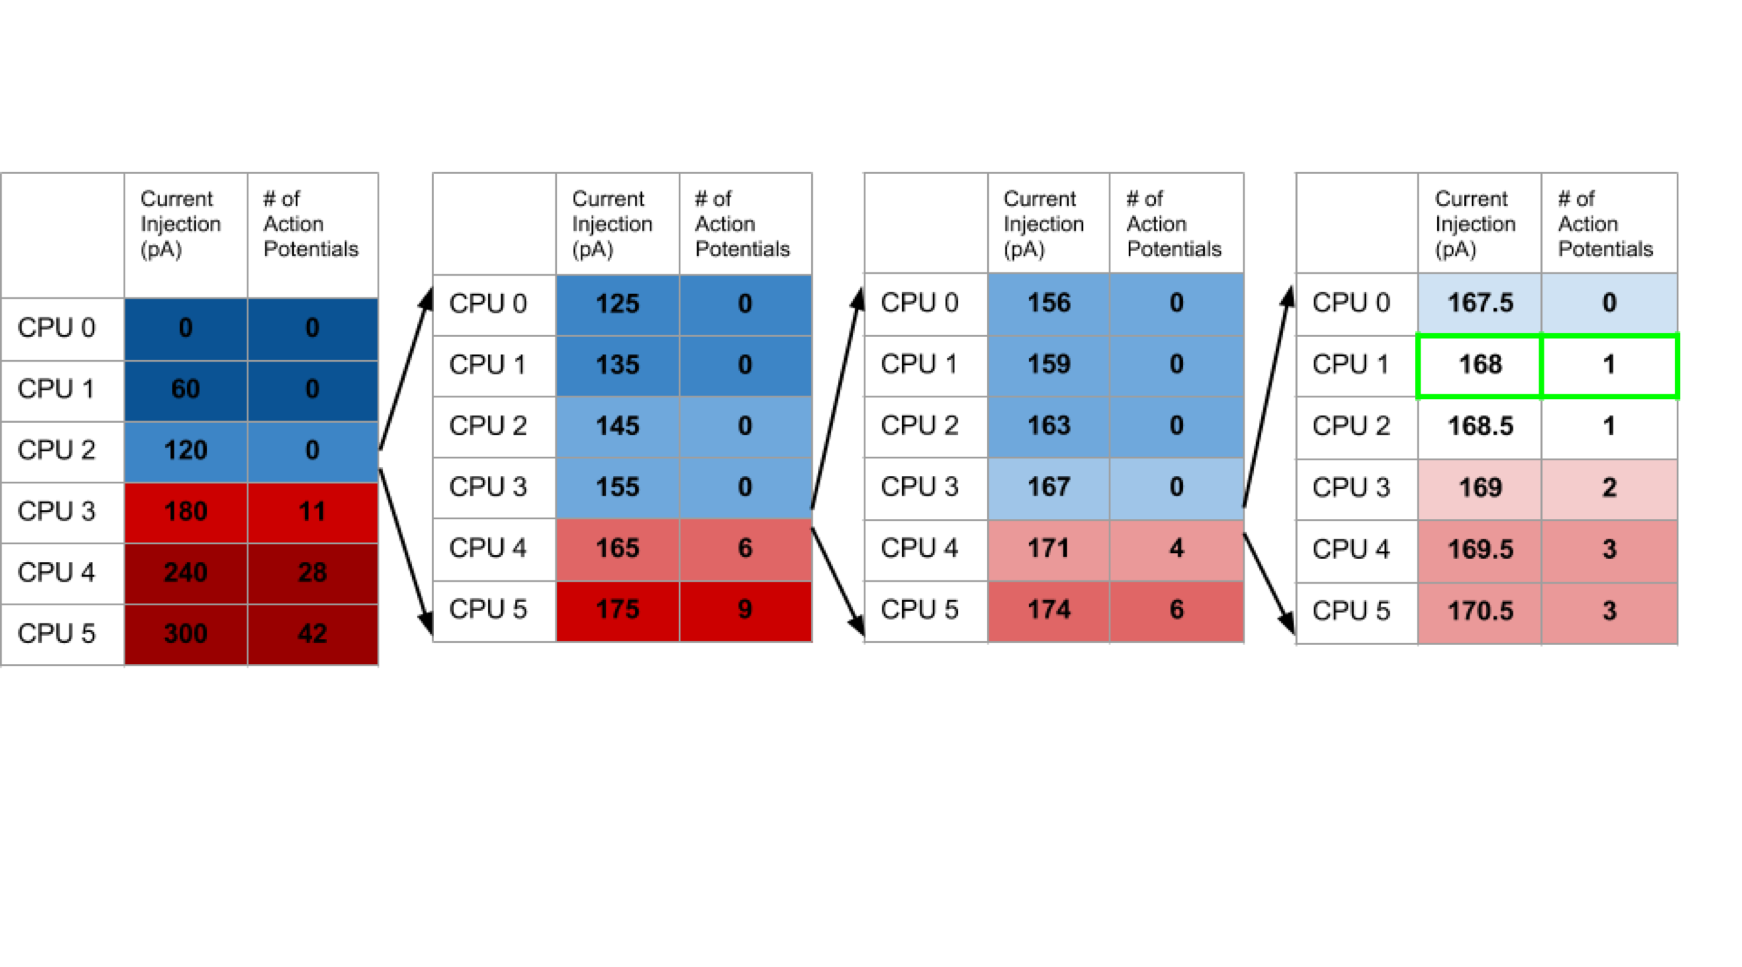
\includegraphics[width=0.7\linewidth]{figures/rheobase_algorithm.png}
\caption{We developed a generic algorithm which took models, and found the minimal current injection value that would cause only one spike. The normal structure of this algorithm is a binary search, however we modified the algorithm so it would map onto multiple processors at once. This lead to significant speed ups for multicompartment NEURON models}

\end{center}
\end{figure}  

\begin{figure}    
\begin{center}
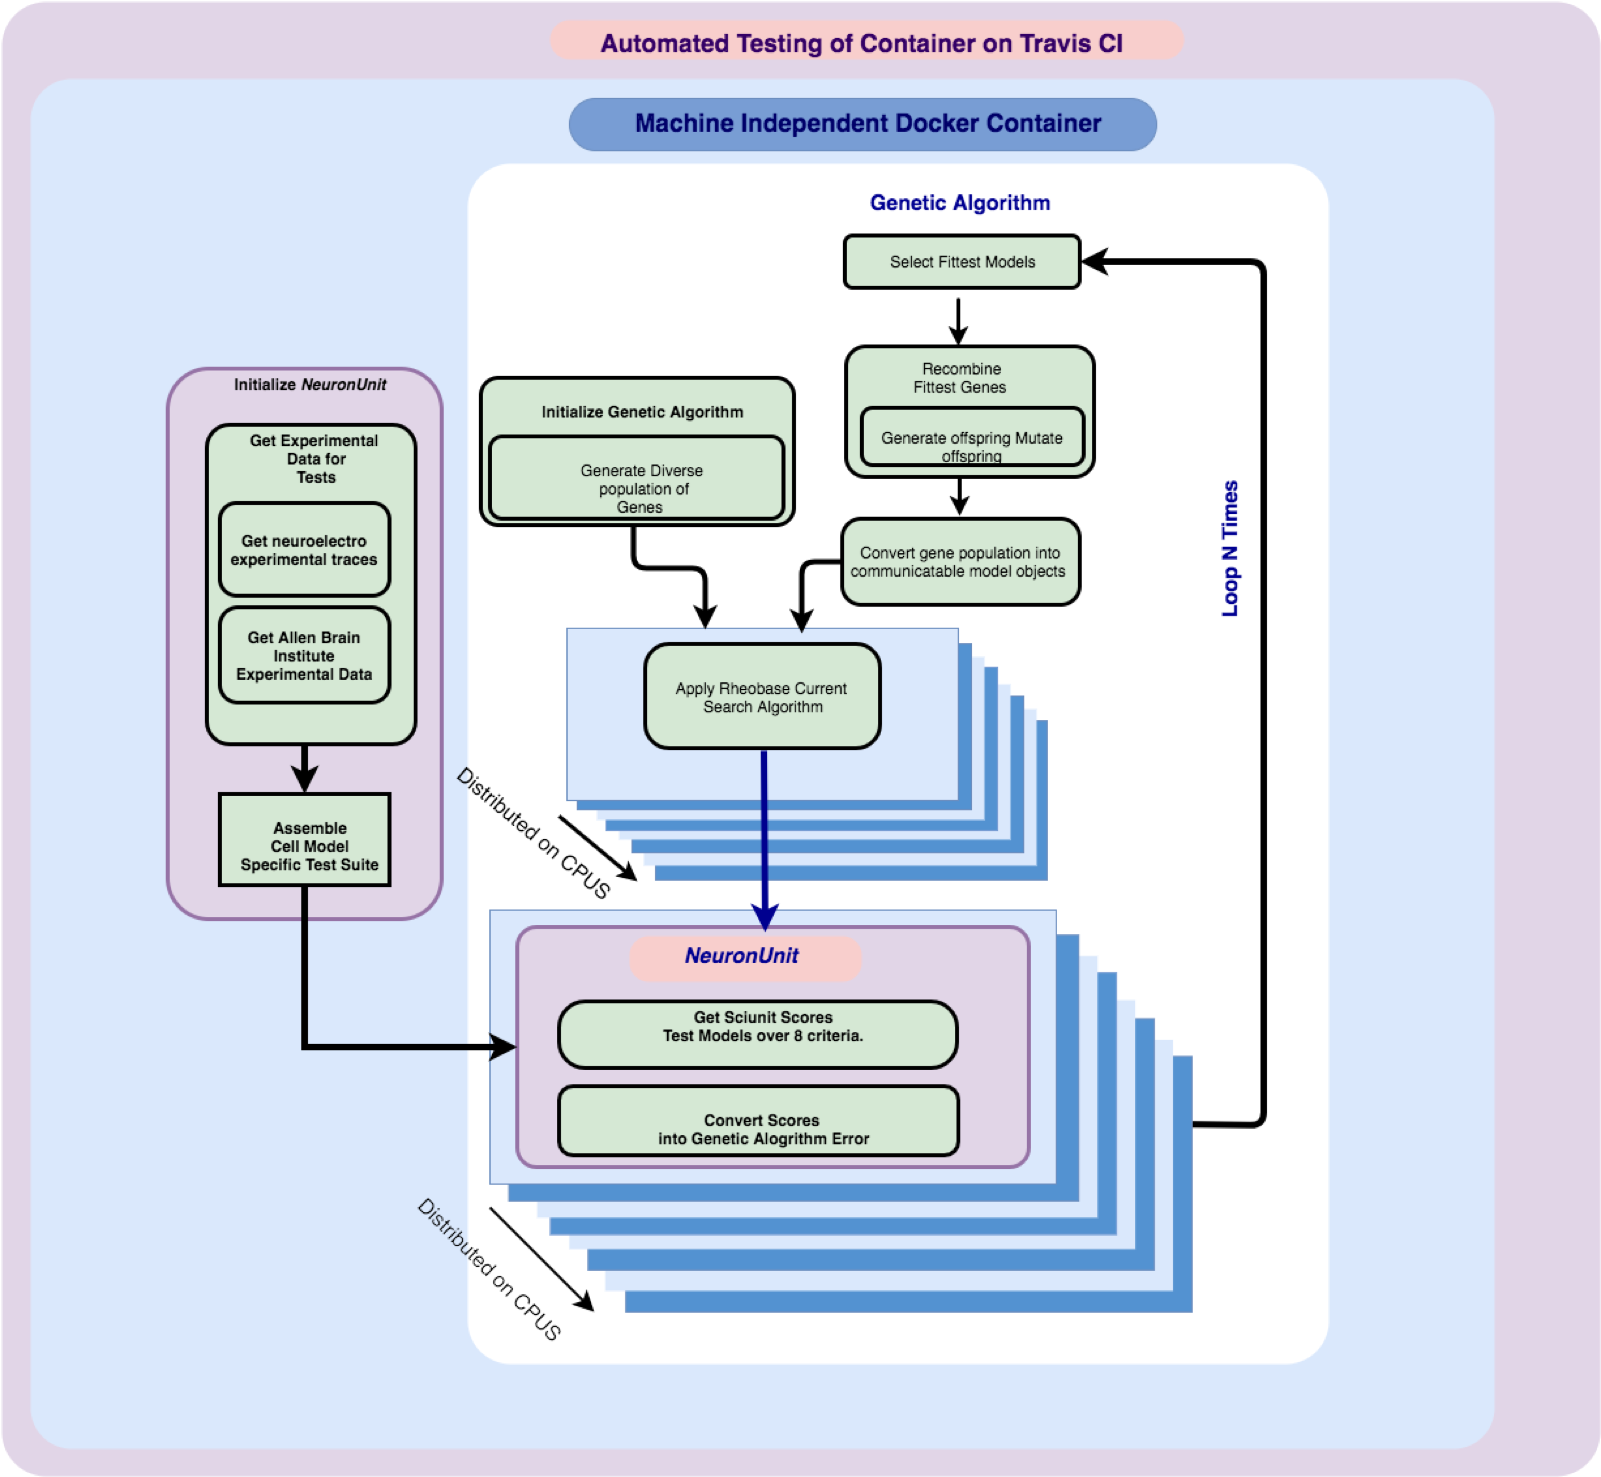
\includegraphics[width=0.7\linewidth]{figures/software_architecture.png}
\caption{In the process of performing the analysis in this work, we expanded an existing neuron model optimisation frame work BluePyOpt \cite{bluepyopt}, by adding in workflows to handle different and elaborate constraint functions and different and elaborate models. and found the minimal current injection value that would cause only one spike. The normal structure of this algorithm is a binary search, however we modified the algorithm so it would map onto multiple processors at once. This lead to significant speed ups for multicompartment NEURON models}

\end{center}
\end{figure}